% !TeX spellcheck=en_GB
\section{Preliminary}

This section contains a small survey of prior related work in the context of parallel Simplex implementations, as well as the theoretical background for the project.

\subsection{Prior work}
Due to the popularity and importance of linear programming solvers, a lot of research has been done on efficient parallel implementations of Simplex and similar algorithms. In [A Parallel Primal–Dual Simplex Algorithm - 2000] by Diego Klabjan, Ellis L. Johnson, George L. Nemhauser, a multi-computer approach was introduced which solved independent parts of Simplex to decrease the number of iterations required to solve the instances.

In [Efficient Implementation of the Simplex Method on a CPU-GPU System - 2011] by Mohamed Esseghir Lalami, Vincent Boyer, Didier El-Baz, a mix of efficient CPU and CUDA routines were used to obtain a 12.5 times speedup of the Simplex algorithm when compared to a purely CPU-based one.

In [Efficient GPU-based implementations of Simplex type algorithms - 2015] by Nikolaos Ploskas and Nikolaos Samaras, GPU-based implementations of the Revised Simplex and Primal Dual Point algorithms showed speedup increases with a factor of up to $181$ compared to a sequential MATLAB implementation.

\subsection{Linear Programming}
A \textit{linear program} (LP) consists of a set of $n$ \textit{variables} and $m$ \textit{linear constraints}. The LP specifies an objective function which maximizes or minimizes a linear combination of the variables and their coefficients, subject to the $m$ constraints. All variables and constraints must be linear. To formulate precisely:

\begin{alignat*}{3}
\text{max: } &\sum_{i=1}^{n} c_i x_i\\
\text{s.t }  & \sum_{j=1}^{n} a_{ij} x_j \leq b_i && \text{ for } i=1,2,...,m\\
& x_j \geq 0                         && \text{ for } j=1,2,...,n
\end{alignat*}

The variables can be seen as dimensions in a $n$-dimensional coordinate system and the constraints define a convex feasibility region where the values of the variables satisfy all of the constraints. An extreme point of the region will have a specific objective value and it can be shown that the optimal value of the linear program can be found in such a point.

\begin{figure}[H]
	\centering
	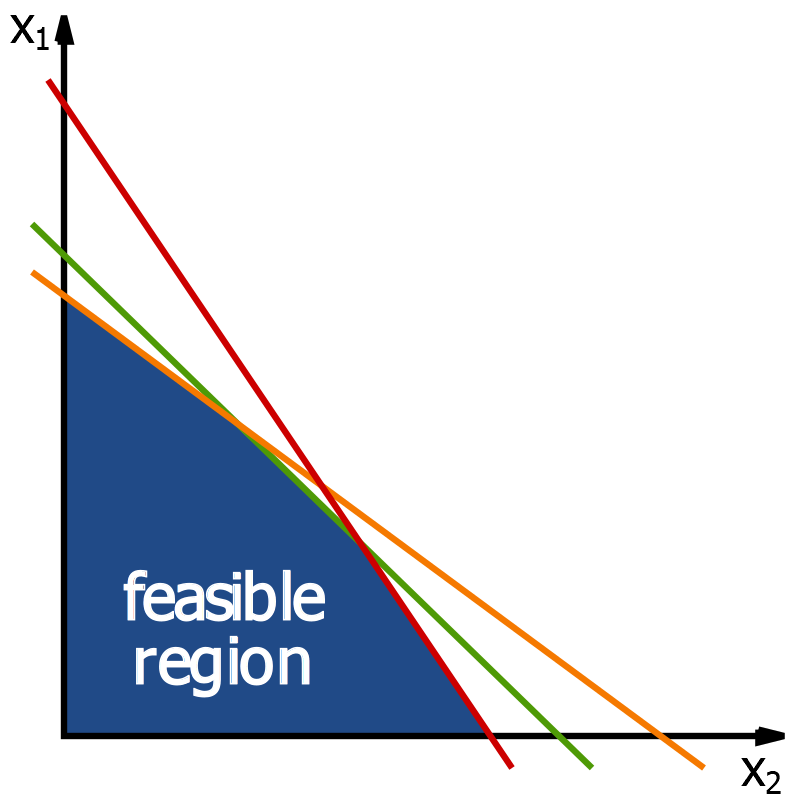
\includegraphics[width=0.6\textwidth]{Linear_Programming_Feasible_Region}
	\caption{The graphical interpretation of a linear program with two variables and three constraints. Source: \url{https://en.wikipedia.org/wiki/Feasible_region}}
	\graphicspath{dir-list}
	\label{key}
\end{figure}

There can be multiple optimal solutions to a linear program, so to validate the correctness of the result, typically only the value of the objective function is used.

\subsubsection{The Simplex Algorithm}
Simplex is a specific algorithm for solving linear programs. It finds the optimal solution by traversing the extreme points of the feasible region, continuously increasing the objective value.
Simplex initiates by formulating each constraint as a new variable. In this formulation every variable in the objective function is called the \textit{non-basic} variables and the new variables of the constraints are called the \textit{basic} variables. Every non-basic variable always has value 0, and every basic variable is therefore equal to the constant of the corresponding constraint. The formulation is as follows:

\begin{alignat*}{4}
\text{objective value} &= &&0 + \sum_{i=1}^{n} c_ix_i\\
x_{n+i}  		&= && b_i - \sum_{j=1}^{n} a_{ij} x_j  &&& \text{ for } i=1,2,...,m
\end{alignat*}

Simplex iteratively pivots variables to increase the objective value. In a pivot, a non-basic variable called the \textit{entering variable} essentially swaps position with a basic variable called the \textit{leaving variable}. The entering variable is a non-basic variable with a positive objective coefficient, and the leaving variable is based on which constraint is the most binding.

After the pivot, the objective value must either increase or stay the same. When it is not possible to pivot any variables without decreasing the objective value, the optimal solution has been found.

\subsubsection{Representation}
One way to represent the constraints and variables is with vectors and matrices. Since we have $n$ variables, the coefficients of the variables can be encoded in a vector $c$ of length $n$. There are $m$ constants of the constraints which can be encoded into a vector $b$ of length $m$. The constraints can be seen as an $m \times n$-matrix $A$ over every variable and constraint.
	
\begin{table}[H]
	\centering
	\begin{tabular}{|l|l|l|l|l|}
		\hline
		& $x_1$                       & $x_2$                        & $x_3$                       &                            \\ \hline
		& \cellcolor[HTML]{ECF4FF}10  & \cellcolor[HTML]{ECF4FF}-0.5 & \cellcolor[HTML]{ECF4FF}5.5 &                            \\ \hline
		$x_4$ & \cellcolor[HTML]{FFCCC9}3   & \cellcolor[HTML]{FFCCC9}3    & \cellcolor[HTML]{FFCCC9}0   & \cellcolor[HTML]{9AFF99}10 \\ \hline
		$x_5$ & \cellcolor[HTML]{FFCCC9}-10 & \cellcolor[HTML]{FFCCC9}0    & \cellcolor[HTML]{FFCCC9}-7  & \cellcolor[HTML]{9AFF99}17 \\ \hline
	\end{tabular}
	\caption{Matrix representation of a linear program with three variables and two constraints. The red cells correspond to the matrix $A$, the green to vector $b$, and the blue to vector $c$.}
	\label{my-label}
\end{table}
